\documentclass{standalone}
\usepackage{tikz,color}
\begin{document}

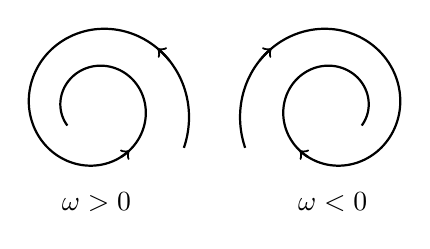
\begin{tikzpicture}
\draw [thick, domain=-4.2:-1.8, samples=100] 
		plot({exp(0.2*\x)*sin(2*\x r)},{exp(0.2*\x)*cos(2*\x r)});
\draw [<-, thick, domain=-1.9:0.5, samples=100] 
		plot({exp(0.2*\x)*sin(2*\x r)},{exp(0.2*\x)*cos(2*\x r)});
\draw [<-, thick, domain=0.4:1, samples=100] 
		plot({exp(0.2*\x)*sin(2*\x r)},{exp(0.2*\x)*cos(2*\x r)});
\node at (0,-1.2) {$\omega>0$};

\draw [thick, domain=-4.2:-1.8, samples=100] 
		plot({3-exp(0.2*\x)*sin(2*\x r)},{exp(0.2*\x)*cos(2*\x r)});
\draw [<-, thick, domain=-1.9:0.5, samples=100] 
		plot({3-exp(0.2*\x)*sin(2*\x r)},{exp(0.2*\x)*cos(2*\x r)});
\draw [<-, thick, domain=0.4:1, samples=100] 
		plot({3-exp(0.2*\x)*sin(2*\x r)},{exp(0.2*\x)*cos(2*\x r)});
\node at (3,-1.2) {$\omega<0$};

\end{tikzpicture}
\end{document}
